\section{Konzept}
Hier wird ein Konzept mit Mock Ups und Architektur entstehen
\subsection{Priorisierung der Erfassungsmöglichkeiten}
\subsectionauthor{Lukas Seemann}
Im Anschluss an die Auswahl der Erfassungsmöglichkeiten werden diese Möglichkeiten nun priorisiert. In der folgenden Tabelle (Tabelle 1) ist die Priosierung abgebildet. \newline
\begin{table}[h]
	\centering
	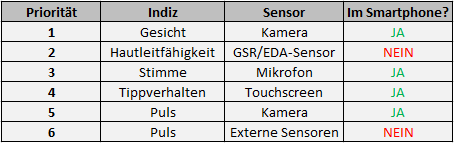
\includegraphics[width=16cm]{Bilder/prio.png}
	\caption[Priorisierung der Erfassungsmöglichkeiten]{Priorisierung der Erfassungsmöglichkeiten}
\end{table}%
\newline In der ersten Spalte ist die Priorität dargestellt. Je niedriger die Zahl ist, desto höher ist die Erfassungsmöglichkeit priorisiert. Die Möglichkeiten werden in der Reihenfolge der hier dargestellten Priorisierung thematisiert und letzten Endes in den Prototyp der mobilen Applikation integriert, um Daten zu erfassen. Je nachdem wie viel Zeit die einzelnen Features benötigen, können mehr und mehr Möglichkeiten der Datenerfassung in die App eingebaut werden, wenn sie noch im Zeitrahmen der Studienarbeit umsetzbar sind. Bei den einzelnen Möglichkeiten werden das Indiz, anhand dessen Rückschlüsse auf eine Emotion gemacht werden kann, und ein Sensor, der Daten zum Indiz für die App erfassen soll, aufgelistet. In der letzen Spalte ist festgehalten, ob der benötigte Sensor in den meisten aktuellen Smartphones bereits enthalten ist oder nicht. \newline
Die höchste Priorität hat die Erfassung des Gesichts mit der Smartphone-Kamera. Grund hierfür ist, dass die Gesichtserkennung sehr genaue Rückschlüsse auf die Emotionen zulässt. Die Ergebnisse liefern außerdem Hinweise für viele unterschiedliche Emotionen, aus welchem Grund die Gesichtserkennung eine gute Basis für die Emotionsbestimmung der mobilen Applikation darstellt. Zusätzliche Indizien können die Ergebnisse der Gesichtserkennung verstärken oder relativieren. Des Weiteren ist vorteilhaft, dass die Erfassungsmöglichkeit ohne externe Sensoren auskommt und lediglich die Smartphone-Kamera genutzt werden kann. 
\newline
Die nächst höhere Priorität hat das Indiz der Hautleitfähigkeit, das mithilfe von GSR- beziehungsweise EDA-Sensoren erfasst werden kann. Diese Art von Sensoren befinden sich wie bereits beschrieben nicht in handelsüblichen Smartphones, weshalb man hierzu einen Arduino verwenden muss, der anschließend Daten an die App weiterleitet. Obwohl dies ein Nachteil ist, wurde diese Erfassungsmöglichkeit so hoch priorisiert, da dies ein Bereich in der App-Entwicklung ist, der nur selten thematisiert wird. Dieses Potenzial ist zusammen mit Aussagekraft der Aktivation zu bestimmten Emotionen der Hauptgrund für die hohe Priorisierung. Jedoch muss die Messung der Hautleitfähigkeit mit einem anderen Erfassungstest kombiniert werden, da die Messung alleine keine eindeutigen Anzeichen für einzelne Emotionen zurückliefert, sondern für mehrere.\newline
An dritter Stelle steht die Stimmerkennung mithilfe des Smartphone-Mikrofons. Obwohl aus der Stimme auch viele Anzeichen für Emotionen herausgelesen werden können und ein Mikrofon in jedem Smartphone integriert ist, hat die Stimmerkennung einen Nachteil. Der Benutzer müsste dazu über eine längeren Zeitraum in das Mikrofon sprechen. Da er das für eine Durchführung der Messung zwingend machen muss, besteht auch die Gefahr, dass die Stimme des User nicht natürlich ist, sondern aufgesetzt ist, da er sich über die Durchführung des Test bewusst ist. Da mit der Gesichtserkennung außerdem bereits eine umfangreiche Basis für die Emotionsbestimmung vorhanden ist, erfolgt die Priorisierung auf Platz 3. \newline
Auf dem vierten Platz folgt die Erfassung des Tippverhaltens mit dem Touchscreen beziehungsweise mit der eingeblendeten Tastatur des Smartphones. Hier ist der selbe Nachteil vorhanden wie bei der Stimmerkennung. Der User muss über eine längere Zeit Eingaben über den Touchscreen vornehmen und er ist sich nach Start des Tests bewusst, dass seine Eingaben analysiert werden. Deshalb ist das Ergebnis des Tippverhaltens-Test einfach manipulierbar. Außerdem ist es auch bezüglich der Privatsphäre des Users problematisch, seine eingegebenen Texte zu analysieren. Trotzdem können bei ehrlicher, nicht manipulierter Benutzung des Test interessante Ergebnisse für die Emotionsbestimmung gewonnen werden. \newline
Auf Platz 5 und 6 folgt die Pulsmessung. Da die meisten Erkenntnisse, die mit der Messung des Puls bezüglich Emotionen gewonnen werden können, bereits mit der Hautleitfähigkeits-Messung abgedeckt werden, sind diese beiden Möglichkeit niedrig priorisiert. Die Pulsmessungen können im besten Fall die Ergebnisse des GSR-Sensor bekräftigen, liefern aber neue keine neuen Erkenntnisse. Die Messung mit der integrierten Smartphone-Kamera wird trotz der vermeindlich geringeren Genauigkeit höher priorisiert als die Messung mit dem externen Arduino-Sensor, da dort keine zusätzliche Hardware verwendet werden muss. \newline
Auf den letzten Platz liegt die Messung der Gangart. Obwohl es sich hierbei auch eine Messung biometrischer Daten handelt, können hieraus nur sehr wenige Anzeichen für Emotionen herausgelesen werden. Von allen beschriebenen Methoden liefert diese Möglichkeit den geringsten Nutzwert für die Zwecke der mobilen Applikation. Aus diesem Grund hat die Implementierung dieser Messung die geringste Priorität. \newline
% Zu diskutieren: Eigentlich wäre Reihenfolge Gesicht, GSR, Stimme, Tippverhalten sinnvoller, da im Theorieteil sich herausstellt das nur mit dem Gesicht ein direkter Schluss auf Emotionen möglich ist. 
\subsection{Übertragung biometrischer Daten in Indikatorscores}
\subsectionauthorlong{Lukas Seemann}
Die von den Smartphone-internen und externen Sensoren zurückgeliefert Daten müssen in der App einheitlich verarbeitet werden. Die zurückgelieferten Daten sind unterschiedlich und meistens selbst nicht aussagend. Mit dem im Theorieteil erklärten Hintergrundwissen ist es jedoch möglich, die Daten zu interpretieren. \newline 
Im Umfeld der App soll diese Interpretation mithilfe von Indikatoren geschehen. Ein Indikator ist in diesem Kontext ein Anzeichen, das für die Emotionsbestimmung herangezogen werden kann. Es existieren einerseits Indikatoren, die sich nur für die Bestimmung einer Emotion eignen, und andererseits auch Indikatoren, die für mehrere Emotionen ausschlaggebend sind. Folgende Indikatoren sind für die Umsetzung geplant: 
\begin{itemize}[noitemsep, topsep=0pt]
	\item activation,
	\item happyIndicator,
	\item sadIndicator,
    \item angryIndicator und
    \item suprisedIndicator.
\end{itemize}
\begin{figure}[h]
	\centering
	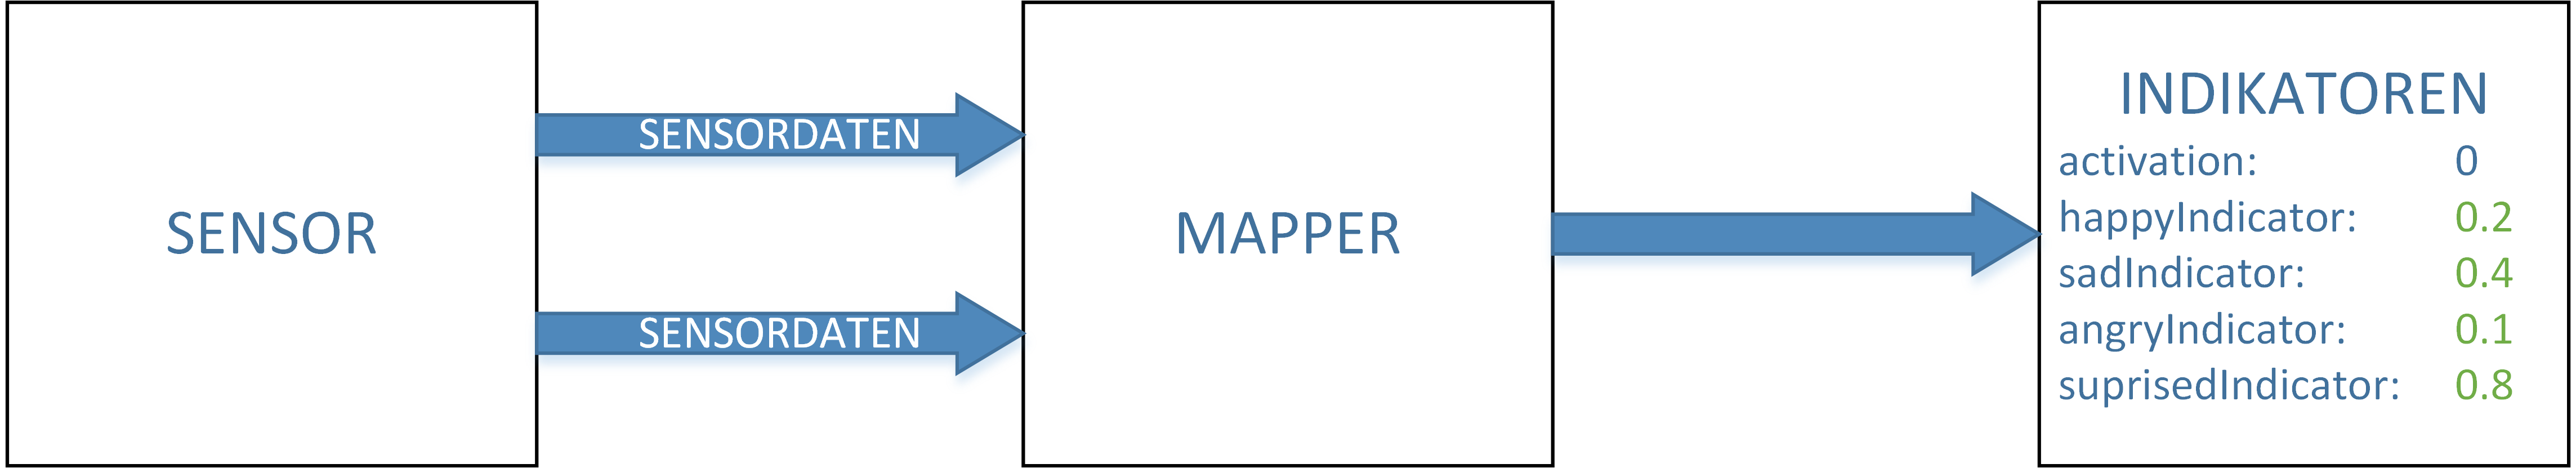
\includegraphics[width=16cm]{Bilder/indicatorscore.png}
	\label{img:Ablauf Erstellung Indicatorscores}
	\caption[Ablauf der Erstellung von Indikatorscores]{Ablauf der Erstellung von Indikatorscores}
\end{figure}%
In Abbildung ? ist der Ablauf der Bestimmung von Indikatorscores abbgebildet. Unabängig davon, welcher Sensor verwendet wird, seine Daten müssen immer auf diese Indikatoren abgebildet werden. Für jeden Sensor muss dabei ein Bereich bestimmt werden, wann immer eine neue Auswertung der Sensordaten zu den sogenannten Indikatorscores geschieht. Eine Auswertung kann generell dann durchgeführt werden, wenn genug Daten vorhanden sind, die aussagekräftig für die Indikatoren sind. Dies ist von Sensor zu Sensor unterschiedlich und muss dementsprechend berücksichitgt werden. \newline
Bei einer Auswertung werden die einzelnen Indikatoren mit Scores von null bis eins versehen, sodass man pro Auswertung der Sensordaten mehrere Indikatorscores erhält. Die Logik für das Setzen der Indikatorscores muss mithilfe von Mappern umgesetzt werden. Für jeden Sensor muss dafür ein individueller Mapper existieren. Die Mapper werden immer dann aufgerufen, wenn genügend Daten des Sensors vorhanden sind. \newline
\subsection{Auswertung der Indikatorscores zur Emotionsbestimmung}
\subsectionauthorlong{Lukas Seemann}
Aus den angesammelten Indikatorscores muss nun entschieden werden, welche Emotion am wahrscheinlichsten beim Benutzer der App vorliegt. Diese Auswertung der Indikatorscores zu konkreten Emotionen erfolgt mit einer Menge von Kausalitätsregeln. Als Ergebnis wird pro Emotion ein Emotionscore erwartet, der angibt, inwiefern die Emotion beim User zum getesteten Zeitpunkt vorliegt. Anschließend muss geplant werden, in welchem zeitlichen Abstand ein neue Emotionscores angelegt werden.
\subsubsection{Kausalitätsregeln}
\subsubsectionauthor{Lukas Seemann}
Eine Kausalitätsregel erwartet eine Menge von Indikatorscores als Eingabe und wendet basierend auf den Indikatorscores Effekte auf die vorhandenen Emotionscores an. Die Indikatoren werden also je nach ihren Werten in verschiedene Emotionen übersetzt. \newline Eine Kausalitätsregel besteht immer aus einer Bedingung und einer Score-Transformation. Eine Bedingung betrifft einen oder maximal zwei Indikatorscores und legt fest, wann die Score-Transformation der Kausalitätsregel ausgeführt wird. Die Score-Transformation beschreibt Effekte, die auf die Emotionscores angewandt werden. Beispielsweise würde einer hoher Score des Stress-Indikators zu positiven Effekten für die Emotionen happy, angry und suprised führen. In Abbildung ? ist der Ablauf der Ausführung einer solchen Kausalitätsregeln gezeigt. Die Formulierung von realitätsgetreuen Kausalitätsregeln ist ausschlaggebend dafür, wie präzise die Anwendung letzten Endes die Emotionen bestimmmen kann. \newline
\begin{figure}[h]
	\centering
	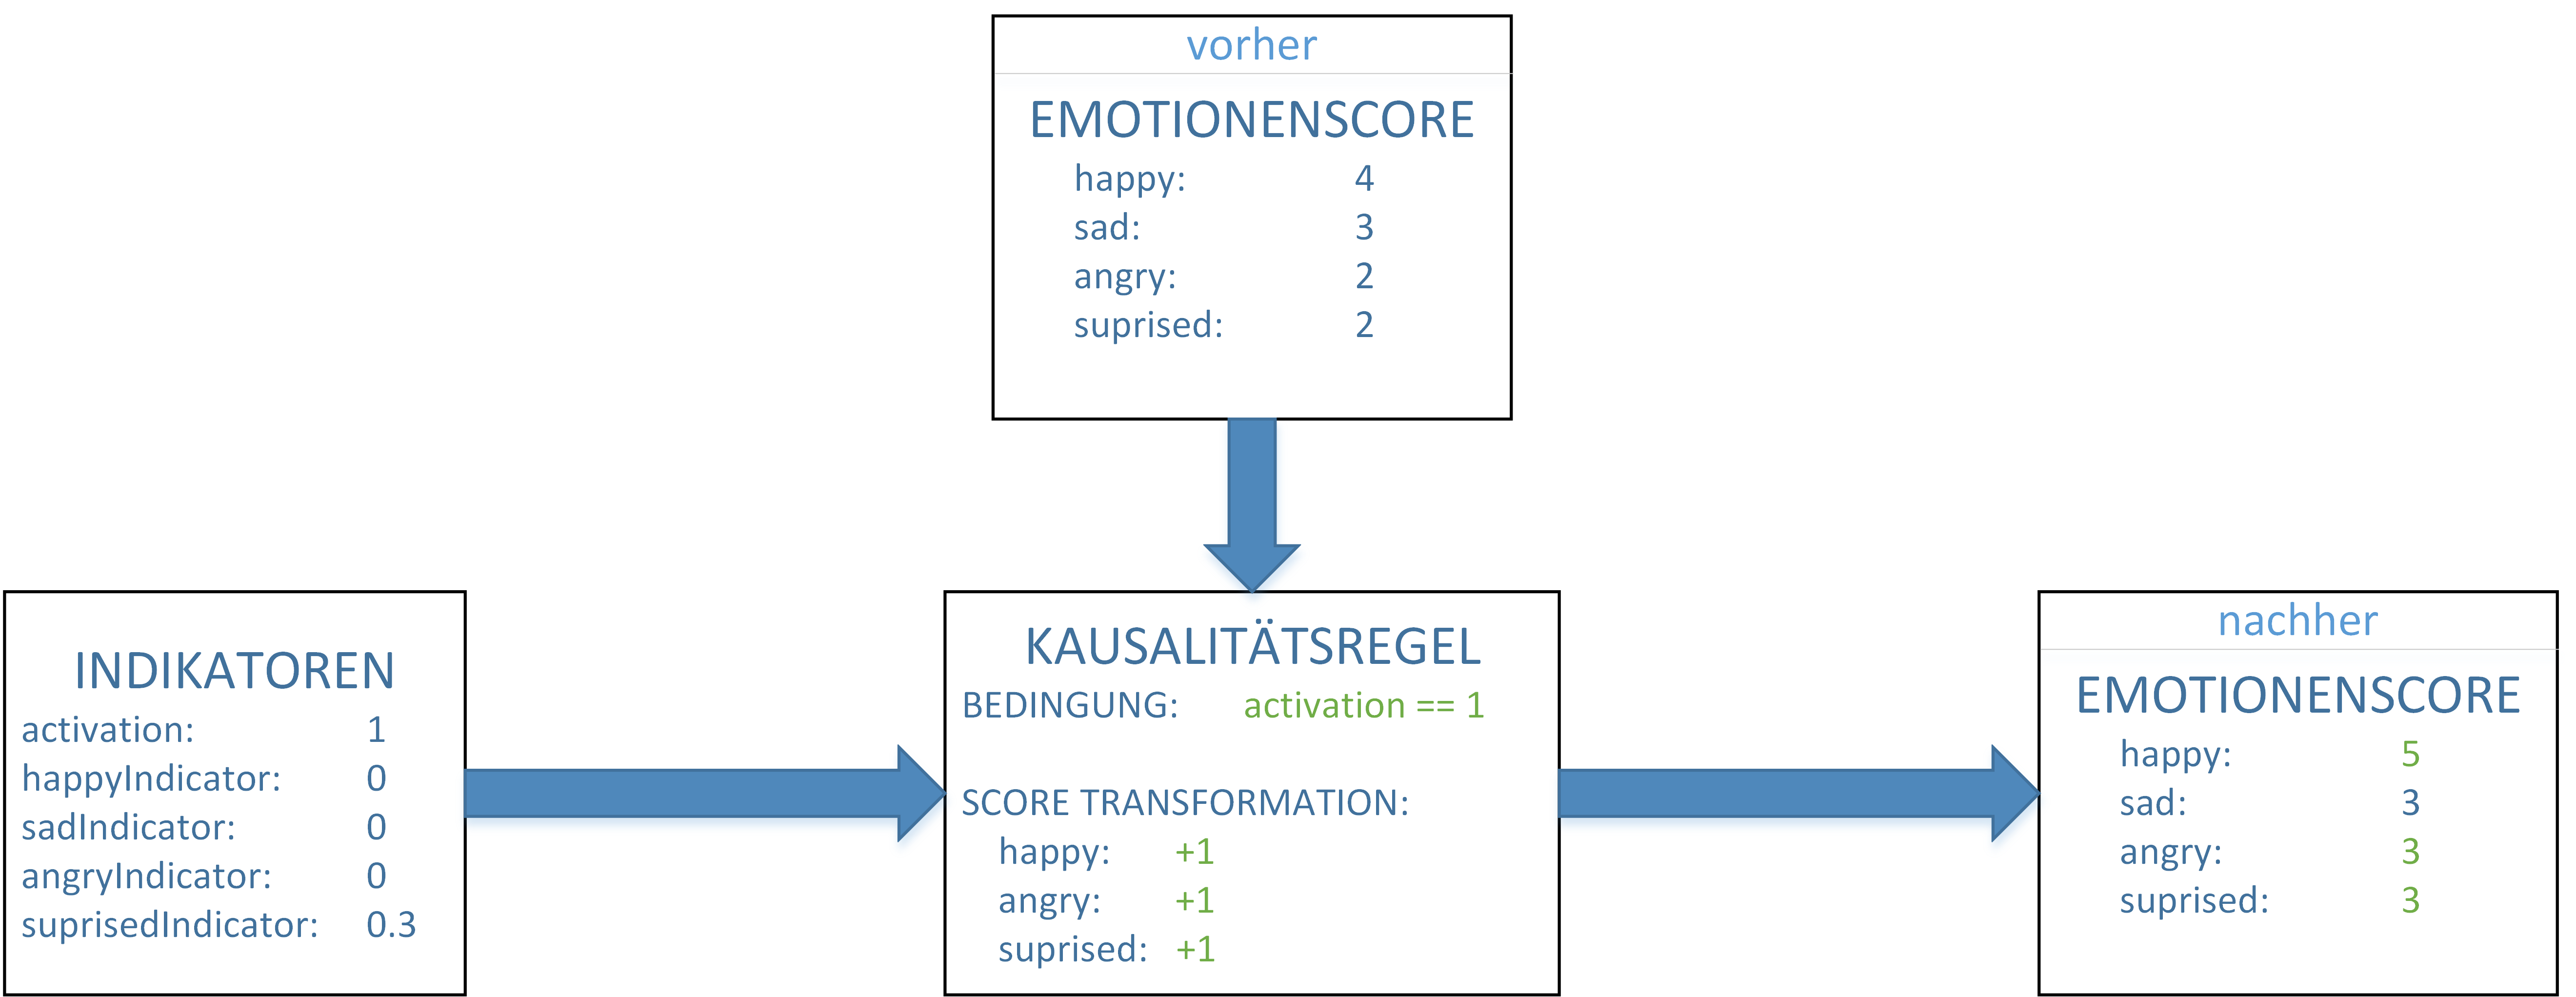
\includegraphics[width=16cm]{Bilder/causalityrules.png}
	\caption[Ablauf der Ausführung von Kausalitätsregeln]{Ablauf der Ausführung von Kausalitätsregeln}
\end{figure}%
\subsubsection{Unterteilung der Entscheidung in Intervalle}
\subsubsectionauthor{Lukas Seemann}
Es wurde bereits beschrieben, wie aus Sensordaten Indikatorscores gewonnen werden und wie wiederum aus diesen mithilfe der Kausalitätsregeln Emotionscores ermittelt werden. Nun muss bestimmt werden, wie oft jeweils neue Emotionscores erstellt und eine Anwendung der Kausalitätsregeln durchgeführt wird. \newline
Um später einen zeitlichen Ablauf der Emotionen des Nutzern anzeigen zu können, muss ein minimaler Zeitbereich bestimmt werden, für den die Auswertung in Emotionscores durchgeführt werden kann. Angedacht ist hierbei, dass der User alle 10 Sekunden ein neue Auswertung erhält. Folglich bedeutet das, dass alle IndicatorScores die in einem 10-Sekunden-Intervall registriert wurden, zusammengefasst werden und für diese dann alle Kausalitätsregeln durchgeführt werden. Dies bedeutet das alle 10 Sekunden ein neue Emotionscores erzeugt werden und anhand der im Intervall vorhandenen Indikatorscores verädert werden. So wird dem User ermöglicht, alle 10 Sekunden eine Bestimmung seiner Emotion in diesem Intervall zu erhalten.
\subsection{Ionic Framework}
In diesem Kapitel wird das Ionic Framework, das für die Umsetzung der mobilen Applikation verwendet wird, vorgestellt und die Gründe für die Verwendung aufgezeigt.
\subsubsection{Aufbau und Einsatz des Frameworks}
\subsubsectionauthor{Lukas Seemann}
Ionic ist ein unter der MIT License stehendes Open-Source-Framework, das zur Entwicklung von plattformübergreifenden, mobilen Applikationen dient. Mit Ionic entwickelte Apps sind damit unter anderem auf Endgeräten lauffähig, die die Betriebssysteme Android, iOS und Windows Phone benutzen. \footcite{Ion18a}
\begin{figure}[h]
	\centering
	
\includegraphics[width=11cm]{Bilder/ionic.png}
	\caption[Ionic Framework - Logo]{Ionic Framework - Logo\footnotemark}
\end{figure}%
\footcitetext{Wik18}
\newline
Aktuell befindet sich das Framework in der Version 3.9.2\footcite[Vgl. ][]{Ion18b} und befindet sich in stetiger Weiterentwicklung. Das Ionic Framework basiert wiederum auf Angular, einem Framework für die Entwicklung von Web-Applikationen. Dementsprechend nutzen Ionic-Anwendungen in der Web-Entwicklung etablierte Technologien wie HTML 5, CSS und JavaScript. \footcite[Vgl. ][]{Ion18c} Wie auch im Angular Framework, wird auch die Programmiersprache TypeScript verwendet, die auf JavaScript aufbaut, sich in der Syntax sehr stark mit JavaScript ähnelt und zusätzliche Optionen zur Typisierung von Variablen oder Funktionen anbietet. \footcite[Vgl. ][]{Til17} \newline
Ionic-Anwendungen sind im Wesentlichen normale Webanwendungen, die von jedem JavaScript-fähigen Browser ausgeführt werden können. Während mithilfe von Ionic das Frontend der Anwendung festgelegt wird, kann anschließend mit Apache Cordova die Plattformunabhängigkeit umgesetzt werden. Apache Cordova bewirkt, dass sich die Webanwendungen wie native Android-, iOS- oder Windows Phone-Applikationen anfühlen. Egal auf welcher Plattform die Ionic-Anwendung installiert wird, es wird die selbe Code-Basis verwendet. Diese wird dann vor dem Installieren von Cordova so angepasst, dass sie auf den Endgeräten ausgeführt werden können. \footcite{Ion18d}
\subsubsection{Gründe für die Verwendung}
\subsubsectionauthor{Lukas Seemann}
Das Ionic Framework bietet eine Möglichkeit mit nur einer Code-Basis, eine plattform-übergreifende Applikation zu erstellen. Dies erspart einiges an Entwicklungsaufwand, da nicht jede Plattform einzeln entwickelt werden muss. Außerdem wird einem Großteil der Smartphone-Nutzer die Nutzung der erstellten App ermöglicht und ist nicht nur für Android- oder Apple-Nutzer beschränkt. \newline
Dadurch dass Applikationen des Ionic Frameworks eigenständige Webanwendungen sind, können diese problemlos von allen Browsern interpretiert und ausgeführt. Dies ist ein großer Vorteil für das Debuggen von Code, da hierfür kein Emulator oder Endgerät verwendet werden muss. Stattdessen kann die Anwendung im Browser ausgeführt und debuggt werden. \newline
Außerdem wurden bereits in anderen Projekten und im privaten Bereiche Erfahrungen mit dem Ionic Framework gemacht, sodass keine Einarbeitung bei den Entwicklungsarbeiten notwendig ist. Dies spart wiederum Zeit, die effektiv für das Entwickeln genutzt werden kann. 
\subsection{Architektur der mobilen Applikation}
In diesem Kapitel wird die Architektur der mobilen Applikation beschrieben. Die Architektur wird in Front- und Backend der App unterteilt.
\subsubsection{Backendlogik}
\subsubsectionauthor{Lukas Seemann}
Zunächst wird explizit auf das Backend beziehungsweise die Hintergrundlogik der App eingegangen. Für das oben beschriebene Konzept bietet sich eine Umsetzung mit Javascript Klassen an, aus welchem Grund ein UML-Diagramm angefertigt werden kann. Dieses ist in Abbildung ? gezeigt. \newline
\begin{figure}[h]
	\centering
	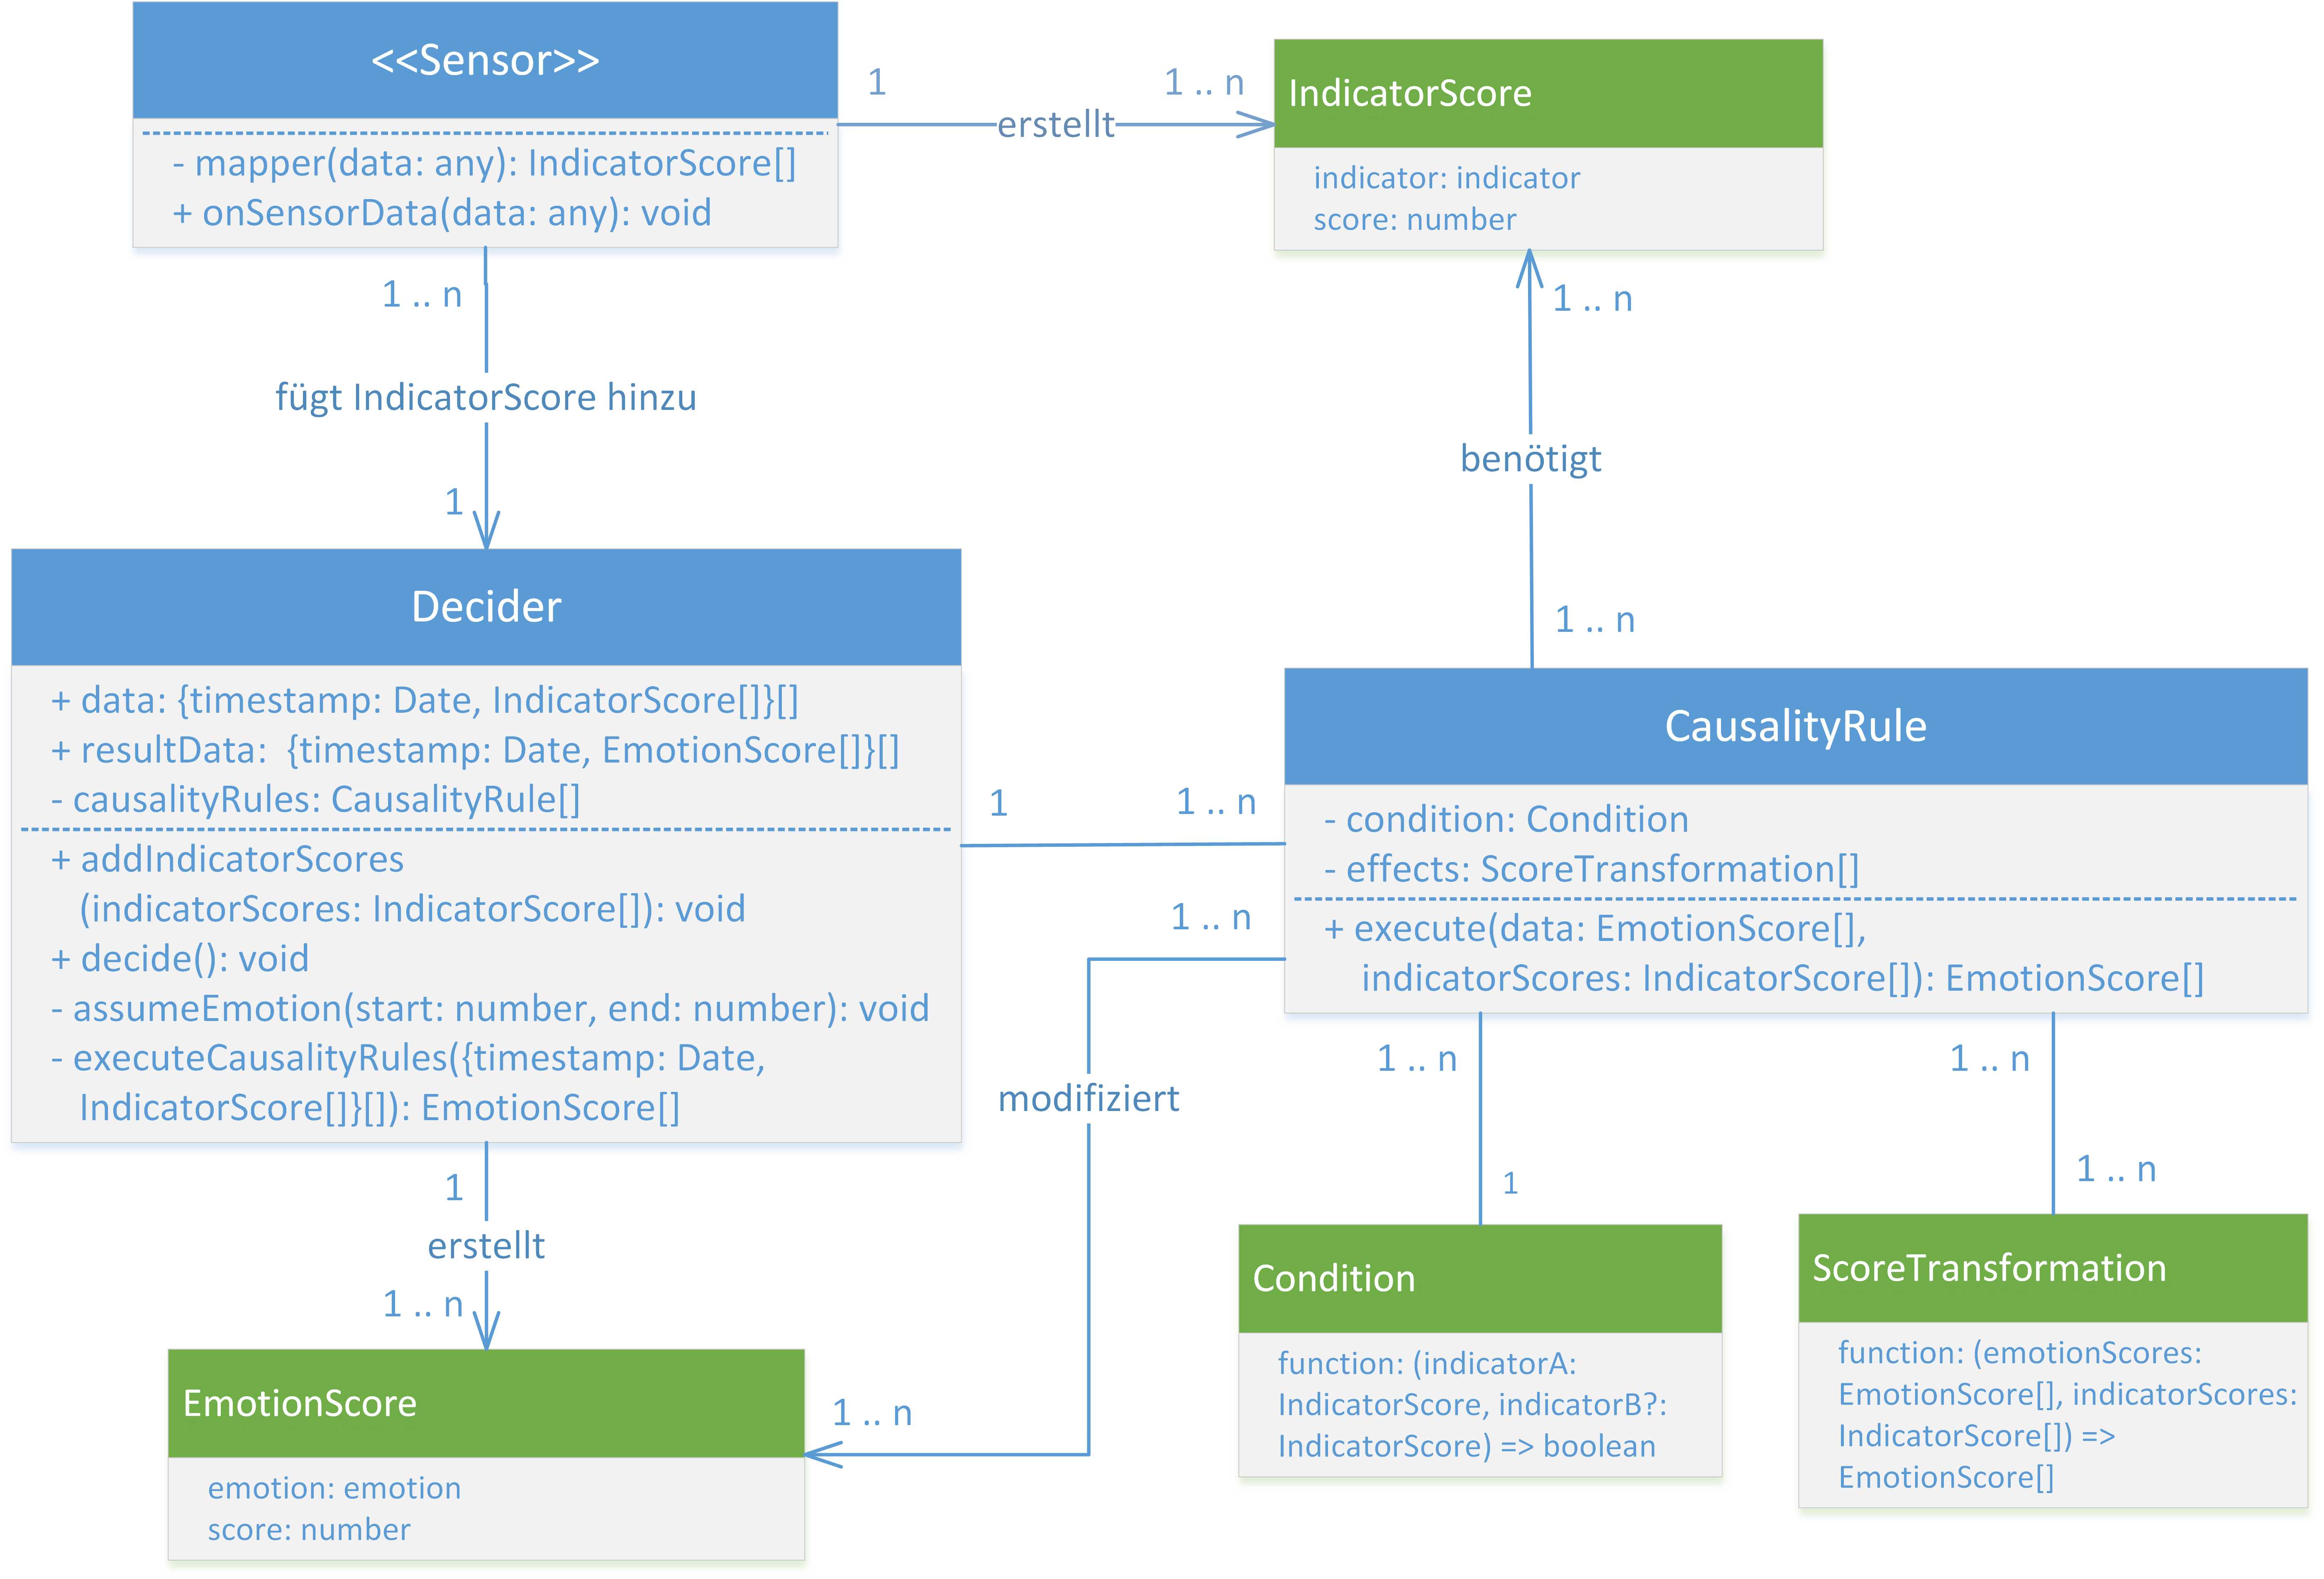
\includegraphics[width=16cm]{Bilder/architecture.png}
	\caption[Architektur der App]{Architektur der App}
\end{figure}%
\newline
Die Klassen sind in der Abbildung blau dargestellt. Typescript bietet die Möglichkeit, eigene Typen zu definieren. Diese Typen verfügen über Attribute, jedoch keine Methoden und sind in der Abbildung grün dargestellt. \newline 
Die App verfügt über eine abstrakte Klasse Sensor, die zwei Methoden definiert. Jeder Sensor, der später Daten für die App liefern soll, muss diese abstrakte Sensor-Klasse erweitern. Dabei muss jeder Sensor die mapper-Funktion überschreiben, die die Sensordaten in mehrere IndicatorScores umwandelt. Auf diese Weise muss jeder Sensor seinen individuellen Mapper implementieren. Der IndicatorScore ist als Typ definiert worden, der einerseits einen Indicator und einen Score als Attribut hat. Indicator wiederum ist ein eigener Typ, der nur die definierten Indikatoren (stress, happyIndicator, sadIndicator, angryIndicator, suprisedIndicator) als String zulässt. Da die Implementierung des IndicatorScore-Types sehr trivial ist, wurde sie aus Übersichtsgründen nicht in die Abbildung aufgenommen. Die onSensorData-Funktion ist bereits vordefiniert und muss dementsprechdend nicht überschrieben werden. Diese Funktion führt lediglich den Mapper aus, wenn genug Sensordaten für eine Auswertung vorhanden sind, und fügt die resultierenden IndicatorScores zum Decider hinzu. \newline \newline
Die Decider-Klasse ist der Hauptbestandteil der App, da sie die Bestimmung der Emotion durchführt. Die Decider-Klasse ist als Singleton anzusehen, da es pro laufende Anwendung nur einen Decider geben kann. Der Decider verfügt über ein data-Array, das allen Input der Sensoren enthält. Konkret handelt es sich hierbei um die Indicatorscores, die die Sensoren ermittelt haben, erweitert mit einem Timestamp für den Zeitpunkt der Ankunft. Nach und nach wird dieses Array mit den IndicatorScores der verschiedenen Sensoren gefüllt. Dies wird mit der Funktion addIndicatorScores() realisiert, die von den Sensoren mit der onSensorData-Funktion aufgerufen wird. \newline
Der Decider verfügt außerdem über ein Array von CausalityRules. Die CausalityRule-Klasse ist die Implementierung der oben beschriebenen Kausalitätsregel. Eine CausalityRule besitzt immer eine Condition (Bedingung) und eine Menge von ScoreTransformationen. \newline
Eine Condition wurde als eigener Typ definiert und ist eine Funktionen, die einen  IndicatorScore (optional auch zwei) als Input hat und auf einen Boolean-Wert abbildet. So kann eine Bedingung realisiert werden, die je nach Erfüllung true oder false zurückgibt. Eine ScoreTransformation ist ebenfalls ein eigener Typ, der eine Funktion definiert. Diese Funktion erhält als Input die vorhandenen Emotionscores, wendet auf diesen Effekte an und gibt die modifizierten Emotionscores zurück. \newline
Die execute-Funktion der CausalityRule führt alle hinterlegten ScoreTransformations aus, wenn die Condition von den IndicatorScores erfüllt worden ist. \newline
Um die Decider-Klasse weiter zu verstehen, muss zunächst der Typ Emotionscore erklärt werden. Dieser ist ähnlich wie der IndicatorScore aufgebaut. Zunächst wird eine Emotion angegeben, die dem Typ Emotion entsprechen muss. Der String muss dementsprechend mit den definierten Emotionen (happy, sad, angry, suprised) übereinstimmen. Anschließend folgt eine Nummer, die den Score angibt.\newline \newline
Die Decider hat ein resultData-Array, das mehrere Emotionscores enthält und die Timestamp der IndicatorScores, aus denen die Emotionscores erzeugt wurden. Dieses Array wird mithilfe der decide-Funktion gefüllt. Wenn die decide-Funktion ausgeführt wird, wird anschließend für alle im data-Array vorhandenen Timestamps die assumeEmotion()-Funktion ausgeführt. Als Parameter erhält diese Methode eine Timestamp und filtert alle IndicatorScores aus dem data-Array zu diesem Zeitpunkt. Für alle auf diese Weise gefilterten Indicatorscores wird anschließend die executeCausalityRules()-Funktion ausgeführt. Diese Funktion wiederum iteriert über alle vorhandenen CausalityRules und führt diese auf Basis der IndicatorScores aus. So erhält man am Ende Emotionscores. Diese erhalten die Timestamp, die bei assumeEmotion() mitgegeben wurde und werden in das resultData-Array gespeichert. Hat man die assumeEmotion-Funktion für alle Timestamps ausgeführt, ist das result-Array komplett gefüllt und die Emotionsbestimmung abgeschlossen.
\subsubsection{Frontend}
\subsubsectionauthor{Lukas Seemann}
Nachdem bereits das Backend beschrieben wurde, wird nun das Frontend der App thematisiert. Unter dem Frontend werden die Screens der App verstanden, die der User bei Nutzung der App aufrufen kann. Diese Screens werden bei Ionic Pages genannt und bestehen meist aus folgenden Bestandteilen: 
\begin{itemize}[noitemsep, topsep=0pt]
	\item Eine Typescript-Datei (.ts), 
	\item eine HTML-Datei (.html) und
	\item eine CSS-Datei (.scss).
\end{itemize}
In der Typescript-Datei wird die Anwendungslogik umgesetzt, außerdem erfolgt dort der Zugriff auf die Backendkomponenten wie zum Beispiel den Decider, die durch das Ionic Framework als sogenannte Provider bereitgestellt werden. Die HTML-Datei beschreibt den Aufbau der GUI der Page, wohingegen die CSS-Datei das Design der Page beschreibt. \newline
In Abbildung ? ist zu sehen, über welche Pages die App verfügen soll, welchen Zweck diese haben und wie sie miteinander in Verbindung stehen.
\begin{figure}[h]
	\centering
	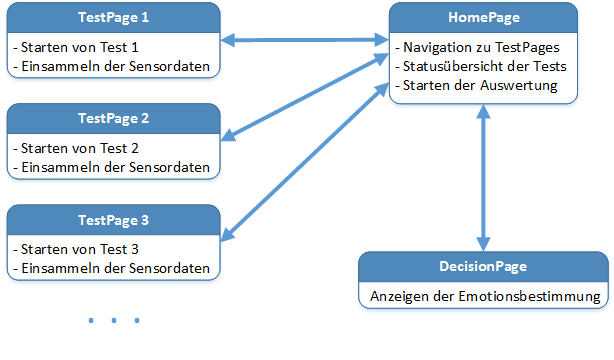
\includegraphics[width=15cm]{Bilder/frontend.png}
	\caption[Geplantes Frontend der App]{Geplantes Frontend der App}
\end{figure}% 
\newline
Für die App sollen nach und nach sogenannte Emotionstest entwickelt werden. Unter einem Emotionstest versteht man im Kontext dieses Projekts die Messung eines Sensors, die Rückschlüsse auf die Emotion zulassen. Ein Emotionstest liefert aus Backend-Sicht immer eine Menge von Indikatorscores zurück. Pro Emotionstest muss eine Page der App angelegt werden, auf der der Test gestartet werden kann und so die Sensormessdaten eingesammelt werden können. \newline
Zwangsläufig verfügt die App über eine HomePage, auf die der User beim Starten der App gelangt. Über diesen Screen kann der User zu den einzelnen TestPages gelangen, um die Tests durchzuführen. Von den TestPages kann der User entweder durch Abschließen der Tests oder durch manuelles Navigieren und Unterbrechen des Test zurück zum Homescreen gelangen. Um dem User anzuzeigen, welche Test er schon durchgeführt hat, wird außerdem eine Statusübersicht zu den Tests auf der HomePage zu sehen sein. Des Weiteren muss der User die Möglichkeit haben, die Auswertung der Indicatorscores zu Emotionen starten zu können. Wählt der User diese Option, werden alle Indicatorscores, die sich zu diesem Zeitpunkt im data-Array des Deciders befinden für die Auswertung verwendet. \newline
Für das Ergebnis der Auswertung und somit die Emotionsbestimmung muss ebenfalls eine eigene Page existieren, worauf der User nach Abschluss der Auswertung gelangt. Der User kann von diesem Screen wieder zurück zum Homescreen gelangen, um erneut Emotionstests zu starten. 
\subsubsection{Vor- und Nachteile der Architektur} 
\subsubsectionauthor{Lukas Seemann}
In diesem Abschnitt werden die Vor- und Nachteile der vorgestellten Architektur gegenübergestellt werden. \newline
Ein Vorteil der Architektur ist es, dass beliebige viele Sensoren und somit Emotionstest hinzugefügt werden können, ohne dass das Backend abgeändert werden müsste. Neue Sensoren müssen lediglich, dass Sensor-Interface implementieren und folglich die mapper-Funktion überschreiben. So kann die App in Zukunft beliebig erweitert werden. \newline
Ein weiterer Vorteil ist, dass die Auswertung der IndicatorScores zu Emotionscores zentral über die Kausalitätsregeln verwaltet werden kann, deren Aufbau bereits vorgegeben ist. Da die Kausalitätsregeln ausschlaggebend für die Emotionsbestimmung sind, müssen diese bei Bedarf angepasst werden, wenn Endergebnisse der Emotionsbestimmunf nicht passend sind. Diese Anpassung kann zentral im Array der Kausalitätsregeln geschehen, und es müssen keine Funktionen umgeschrieben werden oder die Architektur abgeändert werden. \newline
Des Weiteren hat die Aufteilung in IndicatorScores und Emotionscores den Vorteil, dass im gesamten Backend eine einheitliche Datengrundlage vorliegt. Da verschiedene Sensoren ganz unterschiedliche Daten zurückliefern, müssen diese vereinheitlicht werden. Dies wurde mithilfe der IndicatorScores und der EmotionScores umgesetzt. Alle Sensoren, die in Zukunft hinzugefügt werden, müssen sich an die Datenstruktur dieser Scores anpassen. Dies wird durch die Mapper und Kausalitätsregeln sichergestellt. \newline
\newline
Ein Nachteil der Architektur ist, dass eine Anpassung der IndicatorScores und der Emotionscores Änderungen an vielen Stellen hervorrufen würde. Will man beispielsweise einen neuen Indikator \textit{disgustIndicator} und eine neue Emotion \textit{disgust} hinzufügen, müssen zunächst alle Funktionen des Deciders angepasst werden, damit diese neue Emotion aufgenommen werden kann. Des Weiteren müssen gegebenenfalls viele vorhandenen Mapper und Kausalitätsregeln angepasst werden, da diese den neuen Indikator beziehungsweise die neue Emotion nicht berücksichtigt haben.
\subsection{MockUps}
\subsectionauthor{Torben Brenner}
Bevor wir mit der Arbeit an dem Prototypen begonnen haben, diskutierten wir zuerst das Design der einzelnen Komponenten der Anwendung. Wir einigten uns darauf, dass die Übersicht über alle Teile des Prototypen auf der Hauptseite des Startbildschirms sein soll (siehe \ref{img:Mockup-Home}).
\begin{figure}[h]
	\centering
	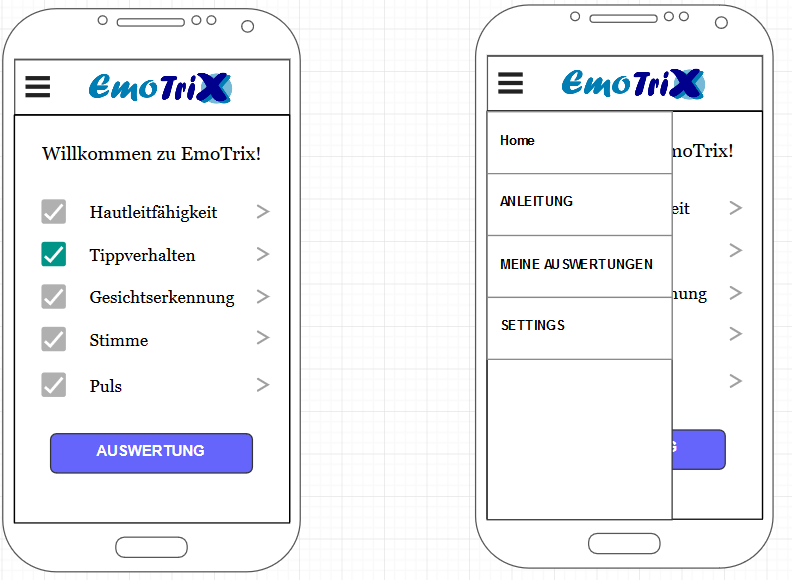
\includegraphics[width=10cm]{Bilder/Mockup-Home.png}
	\label{img:Mockup-Home}
	\caption[Mockup - Homescreen(links) und Menü(rechts)]{Mockup - Homescreen(links) und Menü(rechts)}
\end{figure}%
Wie auf der Grafik zu sehen ist, sind für die fertige Anwendung 5 verschiedene Arten von Tests vorgesehen. Die dazugehörigen Anwendungsabschnitte sollen von der Startseite, durch anklicken des Testnamens aufgerufen werden können und dann ausgeführt werden können. Durch das Berühren des Auswertungsknopfes soll es möglich sein, eine Analyse der verschiedenen Testergebnisse durchzuführen. Diese gibt dann als Ergebnis eine Übersicht heraus, welche Emotionen wie wahrscheinlich sind. Eine Übersicht der bereits durchgeführten Auswertungen soll über das Menü (siehe \ref{img:Mockup-Home} rechts) erreichbar sein. In der Anleitung(ebenfalls über das Menü erreichbar) sollen sich Beschreibungen zur Durchführung der einzelnen Tests befinden.\newline
Im folgenden soll neben den einzelnen Test Seiten, auch die Auswertungsseite genauer beschrieben werden.
\subsubsection{Hautleitfähigkeit}
\subsubsectionauthor{Torben Brenner}
Der Test der Hautleitfähigkeit benötigt die Verbindung mit dem Arduino Microcontroller. Deshalb muss dem Nutzer die Möglichkeit geboten werden, sich mit diesem über die Software möglichst einfach zu verbinden. Hierzu ist eine Seite für die Verbindung vorgesehen\footnote{zu sehen auf der Abbildung Mockup - Arduino verbinden}. 
\begin{figure}[h]
	\centering
	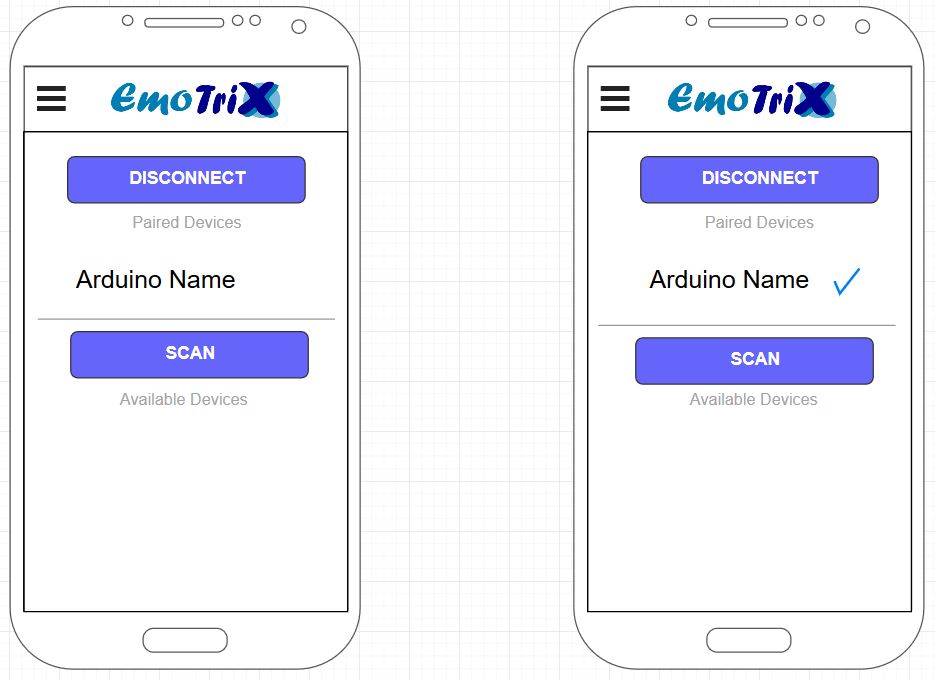
\includegraphics[width=10cm]{Bilder/Mockup-Arduino-Connection.png}
	\label{img:Mockup-Arduino-Connection}
	\caption[Mockup - Arduino verbinden(links nicht verbunden, rechts verbunden)]{Mockup - Arduino verbinden(links nicht verbunden, rechts verbunden)}
\end{figure}%
Auf dieser Seite hat der Nutzer die Möglichkeit, nach verfügbaren Geräten zu suchen. Da der Arduino mittels Bluetooth verbunden wird, werden in der Liste der verfügbaren Geräte auch andere Bluetoothgeräte angezeigt. Bei der Auswahl eines Gerätes wird versucht eine Verbindung mit diesem aufzubauen. Ist dieser Versuch erfolgreich, wird der Name des Gerätes zusammen mit einem Hacken dargestellt. Beim öffnen der Seite ist es ebenfalls möglich, dass der Name des Arduino bereits angezeigt wird. In diesem Fall soll es möglich sein, den Namen zu berühren um eine Verbindung aufzubauen. Gelingt diese wird ebenfalls ein Hacken hinter den Namen gesetzt.\newline
Wo die Verbindung mit dem genau durchgeführt wird, ist noch nicht festgelegt. Denkbar wäre zum einen eine Settingsseite von der aus diese Einstellung erreichbar wäre, zum anderen ist es auch möglich, dass diese Seite angezeigt wird sobald der Test aufgerufen wird.\newline
Der Test ist folgendermaßen aufgebaut. Der Nutzer schließt sich extern an den Hautleitfähigkeitssensor an. Hier sollte die Anleitung genauere Details enthalten wie das zu bewerkstelligen ist. Wenn der Nutzer an den Hautleitfähigkeitssensor angeschlossen ist und mit dem Arduino verbunden ist, kann der Test gestartet werden. Die Messungen beginnen nach dem drücken des Startknopfes. Danach sendet der Sensor über Bluetooth die Daten, welche in Form eines Graphen auf der Oberfläche dargestellt werden\footnote{siehe Abbildung \textit{Mockup - Hautleitfähigkeit Test} auf S.\pageref{img:Mockup-GSR}}. 
\begin{figure}[h]
	\centering
	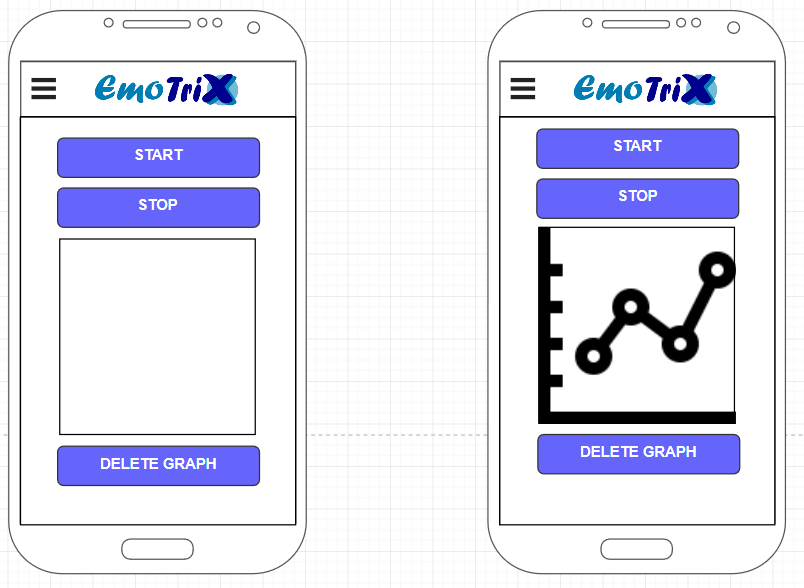
\includegraphics[width=10cm]{Bilder/Mockup-GSR.png}
	\label{img:Mockup-GSR}
	\caption[Mockup - Hautleitfähigkeit Test starten(links) und Test Ergebnis(rechts)]{Mockup - Hautleitfähigkeit Test starten(links) und Test Ergebnis(rechts)}
\end{figure}%
Auf der Seite direkt werden keine Auswertungen der Emotionen dargestellt, sondern nur die Daten des Sensors. Durch betätigen des Stopknopfes, soll die Messung gestopt werden. Mit dem Knopf ``DELETE GRAPH'' wird der gezeichnete Graph zurückgesetzt, aber nicht die bisher erfassten Daten.
\subsubsection{Tippverhalten}
\subsubsectionauthor{Torben Brenner}
Beim Test des Tippverhaltens, ist es angedacht das der Nutzer mit einem ChatBot kommuniziert und die Anwendung im Hintergrund bei Nutzereingaben das Tippverhalten überprüft. In wie fern die Kommunikation mit dem ChatBot abläuft ist noch nicht ganz klar. Es wäre zum denkbar, dass der ChatBot einfach nur einen Dienst zu Verfügung stellt und somit wenig Interaktion bietet. Interessant wäre auch dass vorbereiten eines bestimmten Gesprächs in dem der Nutzer auch von dem ChatBot provoziert werden könnte.
\begin{figure}[h]
	\centering
	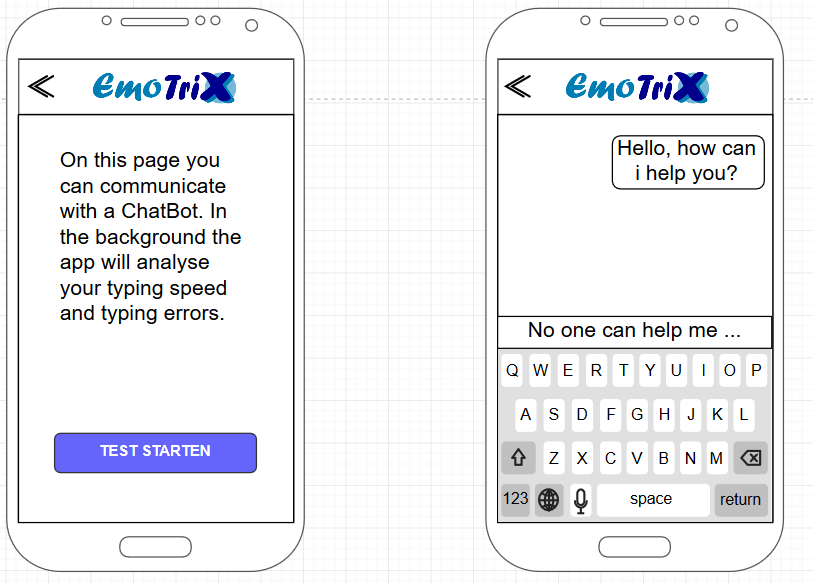
\includegraphics[width=10cm]{Bilder/Mockup-Tippverhalten.png}
	\label{img:Mockup-Tippverhalten}
	\caption[Mockup - Tippverhalten Test starten(links) und Test ergebnis(rechts)]{Mockup - Tippverhalten Test starten(links) und Test ergebnis(rechts)}
\end{figure}% 
Die Oberfläche für die Interaktion mit dem ChatBot soll einem normalen Chat ähneln, d.h. Nachrichten des ChatBots und Antworten des Nutzers werden angezeigt. Der Nutzer bekommt außerdem eine Bildschirmtatstatur angezeigt, auf der er seine Antworten eingeben kann.\newline
Ein Alternative zu diesem Testszenario war, dass der Nutzer einen Zeitraum angibt in dem die App seine Eingaben überwachen darf. Dieser Fall ist aber nicht umsetzbar, da die Betriebssystem natürlich verhindern wollen, dass Passwörter des Nutzers mit gelesen werden können.
Deshalb soll das erste Szenario umgesetzt werden.\newline \newline \newline \newline
\subsubsection{Gesichtserkennung}
\subsubsectionauthor{Torben Brenner}
\label{section:Mockup-Gesichtserkennung}
Bei der Gesichtserkennung wird der Nutzer von der Anwendung dazu aufgefordert, die Kamera zu starten und daraufhin ein Bild mit dieser zu machen. Die Anwendung soll dem Nutzer daraufhin die Aufnahme anzeigen und es ihm ermöglichen das er eine neue Aufnahme machen kann. Wenn der Nutzer eine Aufnahme hat die er analysieren lassen möchte, soll die Anwendung mit Hilfe eines ``Send Picture'' Knopfes die Möglichkeit bieten, dass Bild analysieren zu lassen. \newline
\begin{figure}[h]
	\centering
	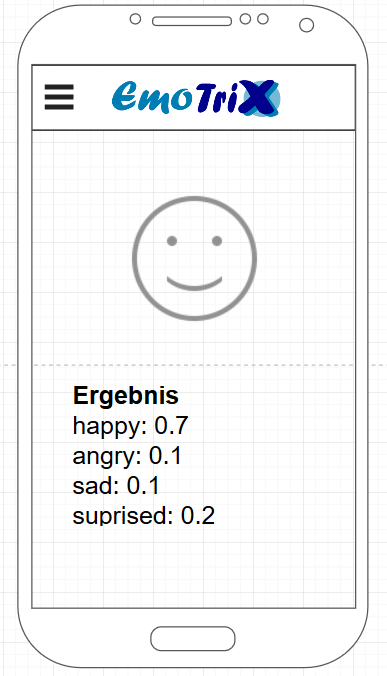
\includegraphics[width=10cm]{Bilder/Mockup-Gesichtserkennung.png}
	\label{img:Mockup-Gesichtserkennung}
	\caption[Mockup - Gesichtserkennung vor Senden des Bilds(links) und Testergebnis(rechts)]{Mockup - Gesichtserkennung vor Senden des Bilds(links) und Testergebnis(rechts)}
\end{figure} \newline
Während der Analyse soll dem Nutzer durch einen Ladebalken signalisiert werden, dass die Daten gerade verarbeitet werden. Auf der Ergebnisseite soll neben dem analysierten Bild das Ergebnis angezeigt werden und außerdem die Möglichkeit bestehen ein neues Bild zu machen oder das gleiche Bild erneut zu analysieren.
\subsubsection{Auswertung}
\subsubsectionauthor{Torben Brenner}
Durch betätigen des Auswertungkopfes auf der Startseite der Anwendung, sollen die bisher erfassten Daten analysiert werden. Das Ergebnis dieser Analyse soll dem Nutzer auf der Auswertungsseite dargestellt werden. Diese besteht aus einem Kreisdiagramm und einem Zeitstrahl.
\begin{figure}[h]
	\centering
	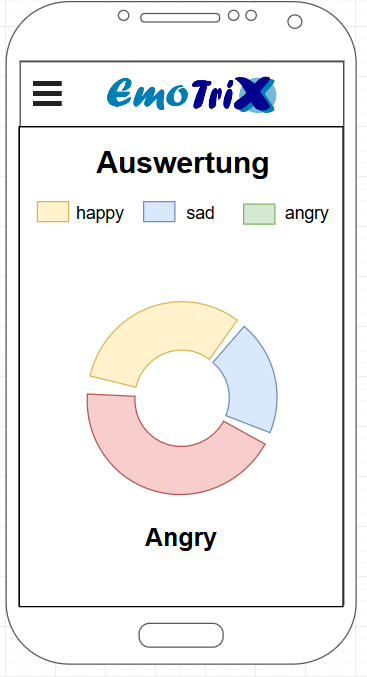
\includegraphics[width=10cm]{Bilder/Mockup-Auswertung.png}
	\label{img:Mockup-Auswertung}
	\caption[Mockup - Auswertung]{Mockup - Auswertung}
\end{figure} \newline
Die Farben des Kreisdiagramms werden durch eine Legende erklärt, d.h. sie werden den einzelnen Emotionen zugeordnet. Durch berühren einer Farbe soll der Nutzer den konkreten Wert für die Emotion angezeigt bekommen. Unter dem Kreisdiagramm soll außerdem ein Zeitstrahl angezeigt werden. Da es später möglich sein soll, Daten im Hintergrund zu erfassen ist es deutlich sinnvoller, die erfassten Daten nicht alle auf einmal zusammen zu rechnen, sondern den Nutzer einen Bestimmten Zeitpunkt auswählen zu lassen. Mit Hilfe des Zeitstrahls soll der Nutzer diese Möglichkeit geboten bekommen.